\documentclass[a4paper,12pt,twoside,openany,Seminar,chapterbib]{ICTv2} % HomePaper or Seminar option
\title{Desulfurization processes and sulfur recovery}
\author{\href{mailto:jayshah4494@gmail.com}{JAY RASESH SHAH}}
\rollno{12CHE1021}
\department{Department of Chemical Engineering}
\college{Institute of Chemical Technology}  %your college
\address{Mumbai -- 400019}
\degree{Bachelors of Chemical Engineering}
\degreedate{2015 -- 2016}    %the degree date
\guide{\textbf{KVM}} %Initials of your guide

\usepackage[svgnames]{xcolor} % Required to specify font color
\usepackage{tfrupee}
\pdfmapfile{=tfrupee.map}

\usepackage{lipsum}

\usepackage{textcomp}

\usepackage{layouts}

\usepackage{epstopdf}

\usepackage[margin=1in]{geometry}

\usepackage{enumitem}

\usepackage{setspace}

\usepackage{amsmath}
\usepackage{amssymb}
%\usepackage{chemfig}
\usepackage{tikz}
\usepackage{caption}
%\usepackage{subfigure}
\usepackage{subfig}
\usepackage[pdfauthor={Jay Shah},pdftitle={Desulfurization processes and sulfur recovery},pdfkeywords={Sulfur, Desulfurization, Sulfur recovery, Claus process, MEROX, biodesulfurization, OATS process},pdfsubject={Seminar 2015-16}]{hyperref} %use [hidelinks] 

\usepackage{booktabs} %fancy tables
\usepackage{float}
\usepackage[intoc]{nomencl} %FOR NOMENCLATURE
\makenomenclature

\usepackage{pdfpages} %to insert external title page pdf

\usepackage{listings}
\usepackage{mcode}

\usepackage{rotating}
\usepackage{pdflscape}

\usepackage[version=3]{mhchem}
\usepackage{multirow}

\usepackage{tablefootnote} %allows footnotes in tables. Duh.
\usepackage{natbib}
\begin{document} 

%\pagestyle{empty} % Removes page numbers
%\renewcommand*{\thepage}{Cover}
%\includepdf{TitlePage.pdf} % includes EXTERNAL title page

\maketitle

\frontmatter
\tableofcontents

\listoffigures
\begingroup
\let\clearpage\relax
\vspace{3em}
\listoftables
\endgroup

\mainmatter
\chapter{Introduction}
\thispagestyle{plain}

Scheduling is a decision-making process that plays an important role in most manufacturing and service industries. %\ref{}. 
Scheduling problems arise in almost any type of industrial production facilities where given tasks need to be processes using specified resources. In a chemical process, production must be planned such that equipment, material and utilities are available at the manufacturing facility when they are needed to realize the production tasks. Production scheduling comprises the activity of planning in detail the production of a product or products in a given production facility. It boils down to the following main decisions \citep{HARJUNKOSKI2014161}:
\begin{itemize}
\item What production tasks to execute?
\item Where to process the production tasks?
\item In which sequence to produce?
\item When to execute the production tasks?
\end{itemize}

For batch processes, short-term scheduling deals with the allocation of a set of limited resources over time to manufacture one or more products following a batch recipe \citep{MENDEZ}. There has been significant development of optimization approaches to scheduling over the last two decades. The first mathematical programming approach the scheduling of multi-purpose, multi-product batch plants was proposed by \cite{KONDILI1993211}. This approach introduces the state task network (STN) representation where the process is described as a bipartite graph consisting of states and tasks.
\chapter{Problem Statement}
\thispagestyle{plain}

The scheduling problem of chemical processes is defined as follows. Given
\begin{enumerate}[label=\roman*.]
\item production recipes (i.e. the processing times for each task at the suitable units, and the amount of the materials required for the production of each product)
\item available equipment and their maximum capacities
\item material storage limitations
\item production requirement
\item time horizon under consideration,
\end{enumerate}
determine
\begin{enumerate}[label=\roman*.]
\item the optimal sequence of tasks taking place in each unit
\item the amount of material being processes at each time in each unit
\item the processing time of each task in each unit
\end{enumerate}
so as to minimize the makespan or maximize the overall profit. \\
There may be sources of uncertainty in the scheduling problem such as:
\begin{enumerate}[label=\roman*.]
\item the processing times of tasks
\item the task yields
\item market demands
\end{enumerate}
The following notation is defined: \\
\textbf{Indices} \\
$i$ = tasks \\
$j$ = units  \\
$s$ = states  \\
$u$ = utilities \\
\textbf{Sets} \\
$\mathcal{J} = $ Set of available processing tasks \\
$\mathcal{S} = $ Set of states (materials) \\
$\mathcal{S} = $ Set of utilities \\
$\mathcal{I} = $ Set of processing tasks \\
$\mathcal{I}_j = $ Set of processing tasks that can be performed in unit $j$\\
$\mathcal{I}_s^p = $ Set of tasks that produce state $s$\\
$\mathcal{I}_s^c = $ Set of tasks that consume state $s$\\
$\mathcal{I}_u = $ Set of tasks that consume utility $u$\\
$\mathcal{I}^{zw} = $ Set of tasks that produce a zero-wait state \\
\textbf{Parameters} \\
$\alpha_i = $ Fixed processing time of task $i$ \\
$\beta_i = $ Processing time of task $i$ per unit batch \\
$\gamma_{iu} = $ Fixed consumption of utility $u$ by task $i$ \\
$\delta_{iu} = $ Consumption of utility $u$ by task $i$ per unit batch \\
$\rho_{is} = $ proportion of state $s$ in the total production/consumption by task $i$ \\
$B_i^{\text{min}} = $ minimum capacity for task $i$ in unit $j$ \\
$B_i^{\text{max}} = $ maximum capacity for task $i$ in unit $j$ \\
$U_u^{\text{max}} = $ maximum availability of utility $u$ \\
$S_{s0} = $ Initial amount of state $s$ \\
$S_{s}^{\text{max}} = $ maximum storage capacity for state $s$ \\
$D_s = $ Demand of state $s$ at the end of horizon \\
$P_s = $ Price of state $s$ \\
$H = $ Horizon




\chapter{Scheduling models used}
\thispagestyle{plain}

\section{CBMN}


\section{MG}


\section{GHM}


\section{IF}


\section{SK}


\chapter{GUI Design}
\thispagestyle{plain}

This chapter describes the basic structure of the instance builder web page and the various assertions and conditions required for a well defined scheduling instance.

\section{Instance structure}
To facilitate compatibility with backend C++ code, the JavaScript instance object is converted to a JSON string. JSON (JavaScript Object Notation) is a text format that is completely language independent but uses conventions that are familiar to many different programming languages, including C, C++, Java, JavaScript, Python and others. These properties make JSON an ideal data-interchange format.

JSON is built on two universal data structures:
\begin{itemize}
\item A collection of name/value pairs. In various languages, this is realized as an object, record, struct, dictionary, hash table, keyed list, or associative array.
\item An ordered list of values. In most languages, this is realized as an array, vector, list, or sequence.
\end{itemize}
Virtually all programming languages support these structures in one form or other. In JSON, they take on these forms:

An \emph{object} is an unordered set of name/value pairs. An object begins with \{ (left brace) and ends with \}  (right brace). Each name is followed by \lstinline{:} (colon) and the name/value pairs are separated by \lstinline{,} (comma).
\section{Instance object}
\label{instanceCompletion}
\begin{figure}[htbp]
\begin{center}
\begin{lstlisting}[xleftmargin=.2\textwidth, xrightmargin=.2\textwidth]
{
	"Name": "Scheduling_Instance",
	"Horizon": 8,
	"Units": [],
	"States": [],
	"Orders": [],
	"Utilities": [],
	"Tasks": [],
	"isCompleteInstance": false
}
\end{lstlisting}\end{center}•
\caption{Instance JSON}
\label{code:Instance}
\end{figure}•
The structure of the Instance JSON object is as shown in Figure \ref{code:Instance}. The empty arrays \lstinline{[]} for \lstinline{"Units"}, \lstinline{"States"}, \lstinline{"Tasks"}, \lstinline{"Utilities"} and \lstinline{"Orders"} in the structure contain the JSON objects as specific to the instance. \lstinline{"Name"} is a string denoting the given name for the instance. \lstinline{"Horizon"} is an integer or float. \lstinline{"isCompleteInstance"} is a boolean \lstinline{true} or \lstinline{false} value denoting if an instance is completely specified.

Figures \ref{fig:unitJSON} - \ref{fig:taskJSON} show the structures of the unit, state, utility, order and task JSON objects respectively.
\begin{figure}[!tbp]
  \centering
  \begin{minipage}[b]{0.4\textwidth}
    \begin{lstlisting}
{
	"Name": "Unit1",
	"MaximumCapacity": 100
}
\end{lstlisting}
    \caption{Unit JSON object}
\label{fig:unitJSON}
  \end{minipage}
  \hfill
  \begin{minipage}[b]{0.4\textwidth}
    \begin{lstlisting}
{
	"StateName": "State1",
	"StateInitialLevel": 100,
	"StateMaxLevel": 100,
	"IsZeroWait": true,
	"IsUIS": false,
	"Price": 10
}
\end{lstlisting}
    \caption{State JSON object}
  \end{minipage}
\end{figure}

\begin{figure}[!tbp]
  \centering
  \begin{minipage}[b]{0.4\textwidth}
\begin{lstlisting}
{
	"Name": "Utility1",
	"MaximumAvailability": 250
}
\end{lstlisting}
    \caption{Utility JSON object}
\label{fig:utilityJSON}
  \end{minipage}
  \hfill
  \begin{minipage}[b]{0.4\textwidth}
\begin{lstlisting}
{
	"StateName": "Product1",
	"Amount": 100
}
\end{lstlisting}
    \caption{Order (demand) JSON object}
  \end{minipage}
\end{figure}

An instance is deemed `complete' if:
\begin{enumerate}
\item At least one valid unit
\begin{itemize}
\item Positive maximum capacity
\end{itemize}
\item At least two states
\begin{itemize}
\item Non-negative maximum capacity
\item Initial level is less than or equal to maximum capacity
\item At least one state with positive initial level
\end{itemize}
\item At least one valid task
\begin{itemize}
\item At least one compatible unit with non-zero processing time (at least one of $\alpha$ or $\beta$ is non-zero)
\item At least one consumed state
\item At least one produced state
\end{itemize}
\item Positive horizon and at least one state to be sold with positive price OR At least one state in demand with positive demand amount
\end{enumerate}



%\subsection{Tasks}
\begin{figure}[htbp]

\begin{lstlisting}[xleftmargin=.2\textwidth, xrightmargin=.2\textwidth]
{
	"TaskName": "Task1",
	"CompatibleUnits": [
		{
		"UnitName": "Unit1",
		"alpha": 5,
		"beta": 1
		}
	],
	"ConsumedStates": [
		{
		"ConStateName": "State1",
		"consRatio": 1
		}
	],
	"ProducedStates": [
		{
		"ProdStateName": "State2",
		"prodRatio": 1
		}
	],
	"ConsumedUtilities": [
		{
		"ConsUtilName": "Utility1",
		"CompUnit": "Unit1",
		"gamma": 2,
		"delta": 0.2
		}
	]
}
\end{lstlisting}
\caption{Task JSON object}
\label{fig:taskJSON}
\end{figure}•


\section{Overall scheduling process flow}
\begin{figure}[htbp]
\centering
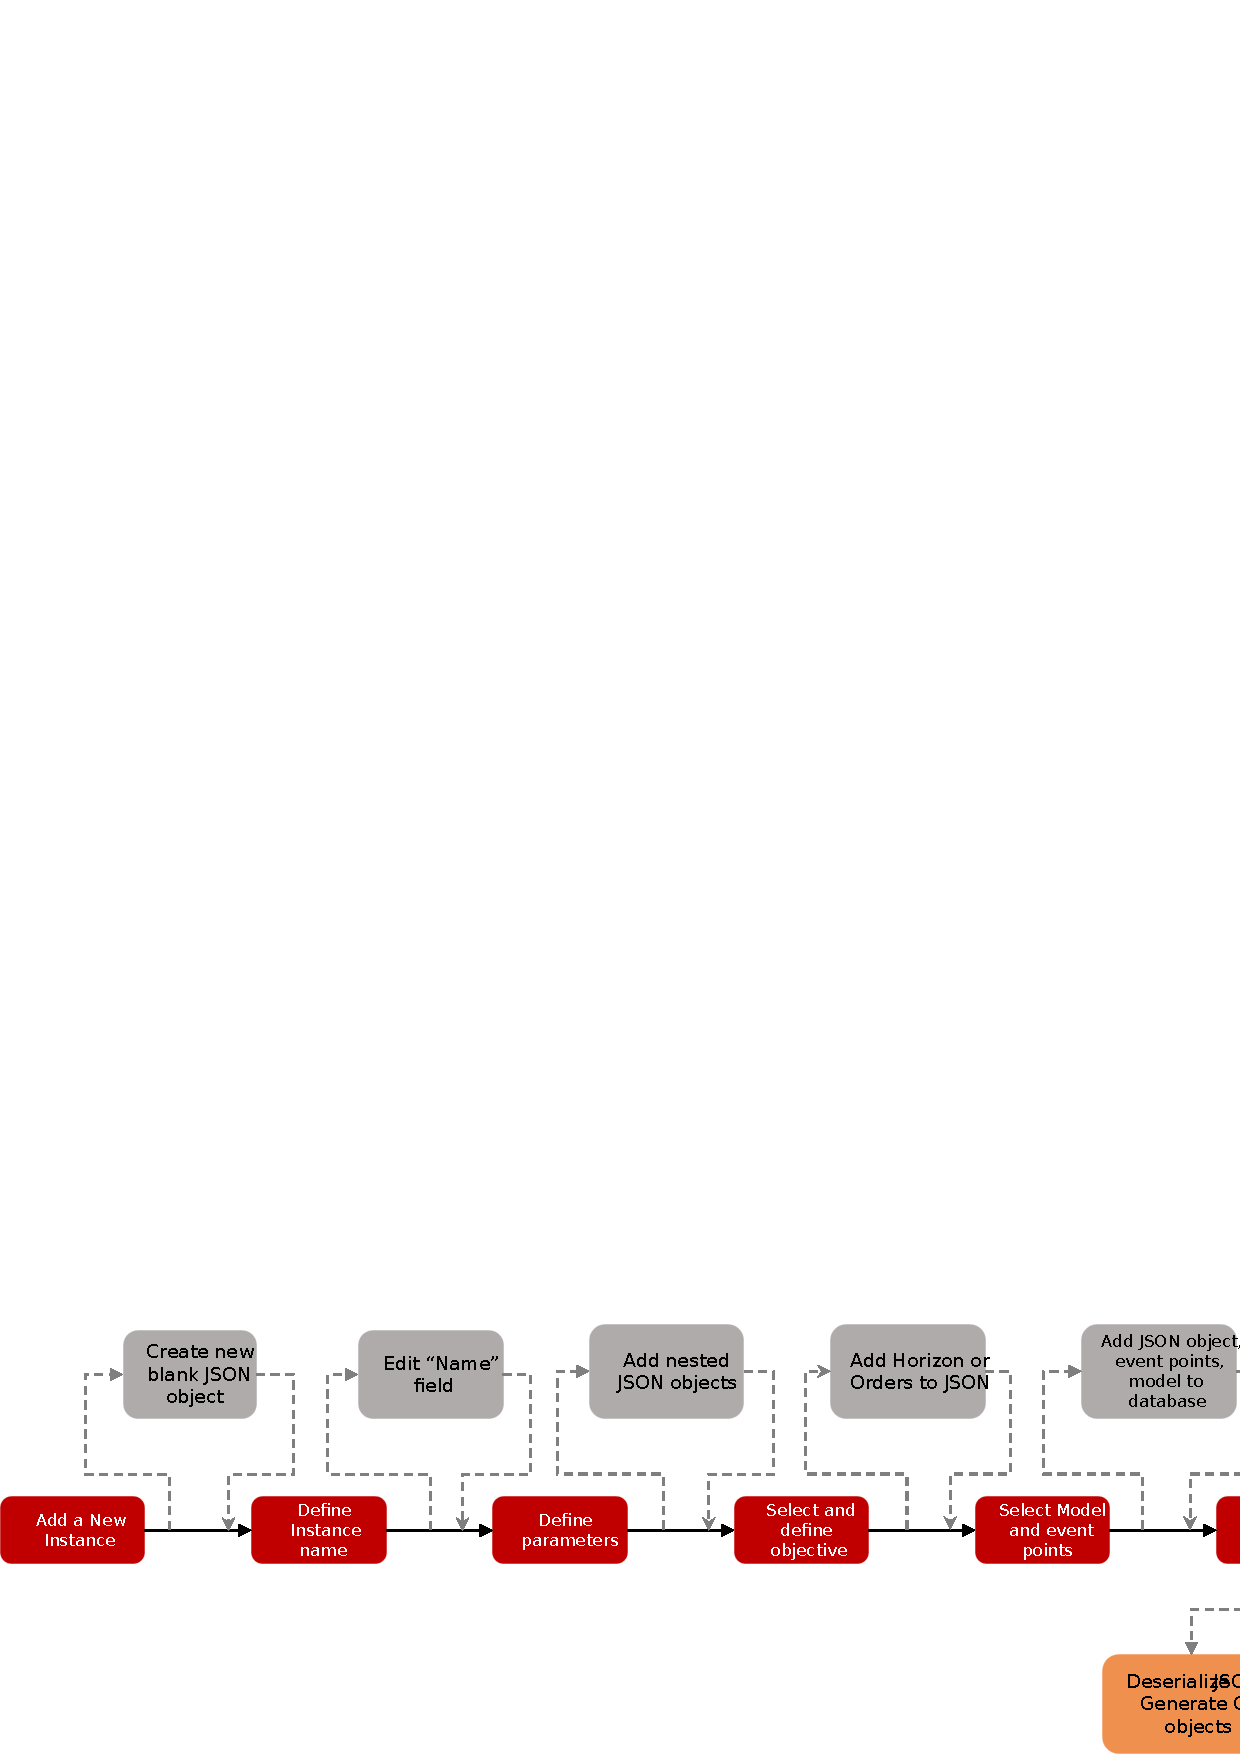
\includegraphics[width=\linewidth]{Images/Communication.png}
\caption{Overall process flow}
\label{fig:Communication}
\end{figure}

Figure \ref{fig:Communication} shows the underlying process behind creating and submitting a scheduling instance. At each stage of the instance building process, the JSON object is converted to a string by means of the \texttt{JSON.stringify()} method in JavaScript and saved in a backend mySQL database. A more detailed process flow for parameter and objective input is shown in Fig. \ref{fig:paraminput}. Once the the instance is complete and amenable to optimization, in the deterministic version, the user has the option of selecting the number of event points and scheduling model to be used. In the uncertain version, the user has additional choices to select uncertain parameters and adjustable variables.

\begin{figure}[htbp]
\centering
\includegraphics[width=\linewidth]{Images/ParameterObjectiveInput.png}
\caption{Parameter and objective input}
\label{fig:paraminput}
\end{figure}

On submitting, a C++ JSON deserializer converts the JSON string to C++ objects. These are then used to build a mixed-integer model in CPLEX according to the model specified by the user.

On successful completion, the following statistics are displayed on the results page:
\begin{itemize}
\item Run time
\item Forumlation
\item Number of event points
\item Objective type
\item Solver status
\item Objective value
\item Number of constraints
\item Number of binary variables
\item Number of continuous variables
\item Number of continuous variables
\item Nodes
\item Root node relaxation
\item Relative gap (\%)
\end{itemize}

If the user has elected to incorporate uncertainty into the instance, the following additional information is displayed:
\begin{itemize}
\item Uncertain Parameter(s)
\item Level of uncertainty
\item Adjustable Variable(s)
\end{itemize}

Additionally, a Gantt chart for the optimal schedule and material inventory charts are displayed. If utilities are specified by the user, then a utility consumption plot is also displayed.

\section{Instance builder}

\begin{figure}[htbp]
\centering
\includegraphics[width=\linewidth]{Images/GUIDesign.png}
\caption[Instance builder elements]{Instance builder elements:
1. Progress bar
2. Instructions
3. Input table
4. Error message(s)
5. Delete item 
6. Drag and drop to rearrange
7. Add new item}
\label{fig:IBGUI}
\end{figure}

Figure \ref{fig:IBGUI} shows the elements in the instance builder GUI. The screenshot in the figure shows the elements in the Units input table. The structure of the States, Utility and Tasks input table follows the same structure. A progress tracker is provided to track the status of the instance being edited. 

Error messages are displayed to ensure that the user input is valid and the instance completion criteria listed in section \ref{instanceCompletion} are satisfied.
 Once a particular set of inputs is completed, clicking on the proceed button will display the next input table.






\section{Submission page}

\begin{figure}[htbp]
\centering
\includegraphics[width=0.8\linewidth]{Images/SelectModelUtilities.png}
\caption{Model selection table for an instance involving utilities}
\label{fig:selectModel}
\end{figure}

On successful completion, an instance becomes available for submission. A screenshot of the model selection table is shown in Fig. \ref{fig:selectModel}. The CBMN 2004 model is selected by default for both the deterministic and uncertain versions. The I\&F 1998 and S\&K 2005 models do not support instances with utilities involved.



\subsection{Uncertainty frameworks}
\begin{table}[htbp]
\centering
\caption{Uncertainty frameworks and  adjustable variables}
\label{tab:adjvars}
\begin{tabular}{@{}cccccc@{}}
\toprule
                  & \multicolumn{2}{c}{Frameworks} & \multicolumn{3}{c}{Adjustable variables} \\ \cmidrule(l){2-6} 
Uncertain parameters   & SRO        & ARO        & \phantom{S } T \phantom{ S}            & \phantom{S } S \phantom{ S}           & B + S       \\ \midrule
$\alpha$          & \checkmark & \checkmark & \checkmark   & \xmark      & \checkmark  \\
$\alpha + \beta$  & \checkmark & \checkmark & \checkmark   & \xmark      & \xmark      \\
$\rho_p$          & \xmark     & \checkmark & \xmark       & \checkmark  & \xmark      \\
$\alpha + \rho_p$ & \xmark     & \checkmark & \checkmark   & \checkmark  & \xmark      \\ \bottomrule
\end{tabular}
\end{table}
If the user elects to incorporate uncertainty in the instance, four types of uncertain variables are available:
\begin{enumerate}
\item Fixed processing time ($\alpha$)
\item Fixed and variable processing time ($\alpha + \beta$)
\item Task yield ($\rho_p$)
\item Fixed processing time and task yield ($\alpha + \rho_p$)
\end{enumerate}

The availability of SRO and ARO frameworks for each of the sets of uncertain variables is shown in Table \ref{tab:adjvars}. If ARO is selected, the uncertain parameters selected dictate the availability of adjustable variables.
\chapter{Case Study}
\thispagestyle{plain}

\section{Instance description}
In this chapter, we present a case study of a well known scheduling instance from \cite{KONDILI1993211}, optimized using the described online tool. The production of two products 1 and 2 from three feed stocks A, B and C takes place according to the STN representation given in Fig. \ref{fig:STN}. This instance has four intermediate states and five tasks.

\begin{figure}[htbp]
\centering
\fbox{\includegraphics[width=\linewidth]{Images/STN.png}}
\caption{State task network for the example instance}
\label{fig:STN}
\end{figure}

Table \ref{tab:statelevels} shows the state maximum capacity and initial load data for the problem. The available unit, task compatibility and processing time data is given in Table \ref{tab:tasks}.

\begin{table}[htbp]
\centering
\caption{Problem data (states)}
\label{tab:statelevels}
\begin{tabular}{@{}cccc@{}}
\toprule
\textbf{State} & \textbf{Capacity} & \textbf{Initial load} & \textbf{Price (per unit)} \\ \midrule
Feed A         & 1000              & 1000                  & -                         \\
Feed B         & 1000              & 1000                  & -                         \\
Feed C         & 1000              & 1000                  & -                         \\
Hot A          & 100               & -                     & -                         \\
Int. BC        & 200               & -                     & -                         \\
Int. AB        & 150               & -                     & -                         \\
Impure E       & 200               & -                     & -                         \\
Product 1      & 1000              & -                     & 10                        \\
Product 2      & 1000              & -                     & 10                        \\ \bottomrule
\end{tabular}
\end{table}

\begin{table}[htbp]
\centering
\caption{Problem data (units \& tasks)}
\label{tab:tasks}
\begin{tabular}{@{}ccccccccc@{}}
\toprule
Unit         & \multicolumn{2}{c}{Heater} & \multicolumn{2}{c}{Reactor 1} & \multicolumn{2}{c}{Reactor 2} & \multicolumn{2}{c}{Separator} \\ \cmidrule(l){2-9} 
Maximum Load & \multicolumn{2}{c}{100}    & \multicolumn{2}{c}{50}        & \multicolumn{2}{c}{80}        & \multicolumn{2}{c}{200}       \\ \midrule
Tasks        & $\alpha$       & $\beta$       & $\alpha$         & $\beta$        & $\alpha$         & $\beta$        & $\alpha$         & $\beta$        \\ \cmidrule(l){2-9} 
Heating      & 0.667        & 0.007       &                &              &                &              &                &              \\
Reaction 1   &              &             & 1.334          & 0.027        & 1.334          & 0.017        &                &              \\
Reaction 2   &              &             & 1.334          & 0.027        & 1.334          & 0.017        &                &              \\
Reaction 3   &              &             & 0.667          & 0.013        & 0.667          & 0.008        &                &              \\
Separation   &              &             &                &              &                &              & 1.334          & 0.007        \\ \bottomrule
\end{tabular}
\end{table}

\section{Adding instance to webtool}
\subsection{Defining units}

Unit names and maximum capacities from Table \ref{tab:tasks} are input into the units table of the web tool as shown in Fig. \ref{fig:defUnits}

\begin{figure}[htbp]
\centering
\includegraphics[width=\linewidth]{Images/DefineUnits.png}
\caption{Units input into webtool}
\label{fig:defUnits}
\end{figure}

\subsection{Defining states}

State names, maximum storage capacities and initial levels from Table \ref{tab:statelevels} are input into the units table of the web tool as shown in Fig. \ref{fig:defStates}.

\begin{figure}[htbp]
\centering
\includegraphics[width=\linewidth]{Images/DefineStates.png}
\caption{States input into webtool}
\label{fig:defStates}
\end{figure}

\subsection{Defining tasks}

This instance does not involve utilities. Hence we can skip utilities input. For each task in Table \ref{tab:tasks}, the values of $\alpha$ and $\beta$ are input after selecting the appropriate compatible unit(s). 

\begin{figure}[htbp]
\centering
\includegraphics[width=\linewidth]{Images/DefineTasks.png}
\caption{Tasks input into webtool}
\label{fig:defTasks}
\end{figure}

%------------------------------------------------------------------------------------------------
% FOR NOMENCLATURE
%------------------------------------------------------------------------------------------------
%1. COMPILE NORMALLY
%2. GO TO CMD PROMPT, CHANGE DIRECTORY TO FOLDER
%3. TYPE makeindex Seminar.nlo -s nomencl.ist -o Seminar.nls
%4. COMPILE AGAIN
%------------------------------------------------------------------------------------------------

%\appendix

%\chapter{Temperature-Enthalpy plot} % Main appendix title

\label{AppendixA} % For referencing this appendix elsewhere, use \ref{AppendixA}

The following program was used to plot the emperature-enthalpy graph in section \ref{sec:tempenthalpy} (Fig. \ref{pinch}):
\lstinputlisting[language=Python]{Appendices/Pinch_v2.py}
%\chapter{Absorption section process flow diagram} % Main appendix title
\begin{figure}[t]
\centering
\fbox{\includegraphics[width=\linewidth]{Images/Absorption.eps}}
\caption{Absorption section}
\label{absorption}
\end{figure}
\label{AppendixB} % For referencing this appendix elsewhere, use \ref{AppendixB}





\backmatter
\def\nomname{Abbreviations}
\printnomenclature[3cm]
%\addcontentsline{toc}{chapter}{Nomenclature}
\newpage

%\singlespacing
\setlength{\bibhang}{7mm}
\bibliographystyle{ICTv2}
\bibliography{Bibliography/bibtexdb}
%\nocite{*}

\end{document}